% Section content template for individual Educative lessons
% This file contains the actual content for a specific section
% Generated from Educative API section content

% Section: Getting Ready: Online Blackjack Game
% Section ID: 5784621407272960
% Section Slug: getting-ready-online-blackjack-game
% Generated: 2025-12-12T12:54:26.651754

\subsection{Problem definition}\label{KfyitG1dioESlbYIcgWus-1}
\\
\textbf{Blackjack} is a popular casino card game where multiple players compete individually against a dealer. The main objective is to have a hand value closer to 21 than the dealer without exceeding it (``busting''). The game uses one or more standard decks of cards. Each card has a specific value: number cards (2-10) are worth their face value, face cards (Jack, Queen, King) are worth 10 points, and the Ace can count as either 1 or 11, whichever benefits the hand most. The best possible hand, a ``Blackjack,'' consists of an Ace and a 10-point card (10, Jack, Queen, or King).
\\
At the beginning of each round, players place bets, and players and the dealer deals two cards to each. Players ' cards are face up, while the dealer has one face up and one face down card. Players can choose to ``hit'' (draw an additional card) or ``stand'' (end their turn) in an attempt to get closer to 21 without busting. If a player's total exceeds 21, they lose immediately. After all players have finished, the dealer reveals their hidden card and draws according to predefined rules. Winners are determined by comparing hand values: the player wins if their total is higher than the dealer's without busting.
\\
In this LLD interview case study, you'll focus on:

\begin{itemize}
\item
\protect\phantomsection\label{6OUmK1f-7d-NY3TcSklxV}
Modeling the core game mechanics of Blackjack, including card values, player and dealer actions (hit, stand), betting, and win/loss conditions.
\item
\protect\phantomsection\label{ZcMDGaUysKVS0r5N7Nwyo}
Designing an interactive flow for multiple players playing concurrently against the dealer, properly handling card dealing, turns, and bet outcomes.
\item
Ensuring the system can reliably manage hands, bets, and game state, while enforcing all Blackjack rules (such as Blackjacks, busts, ties, and dealer drawing rules).
\item
Building a foundation that can be extended for features like multiple tables, different deck sizes, or online multiplayer support.
\end{itemize}
\begin{quote}
\textbf{Note:} This system model is adaptable for online casinos, learning simulators, or any platform looking to provide a scalable Blackjack game experience.
\end{quote}
\\
The following slide represents how to play Blackjack:

\begin{figure}[htbp]
 \centering
 \begin{subfigure}[b]{0.48\textwidth}
 \centering
 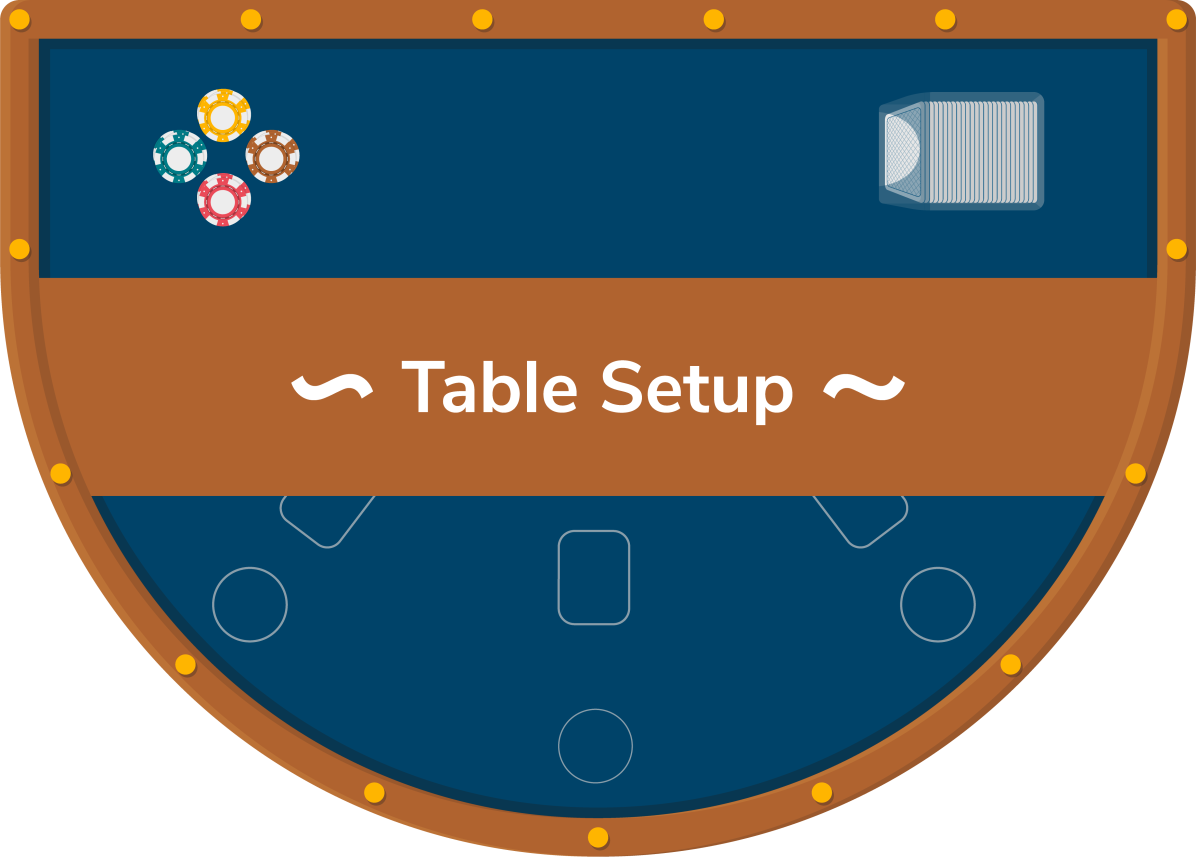
\includegraphics[width=\textwidth]{Images/chapter_12/section_5784621407272960/4987162262241280.png}
 \caption{Blackjack table setup}
 \end{subfigure}
 \hfill
 \begin{subfigure}[b]{0.48\textwidth}
 \centering
 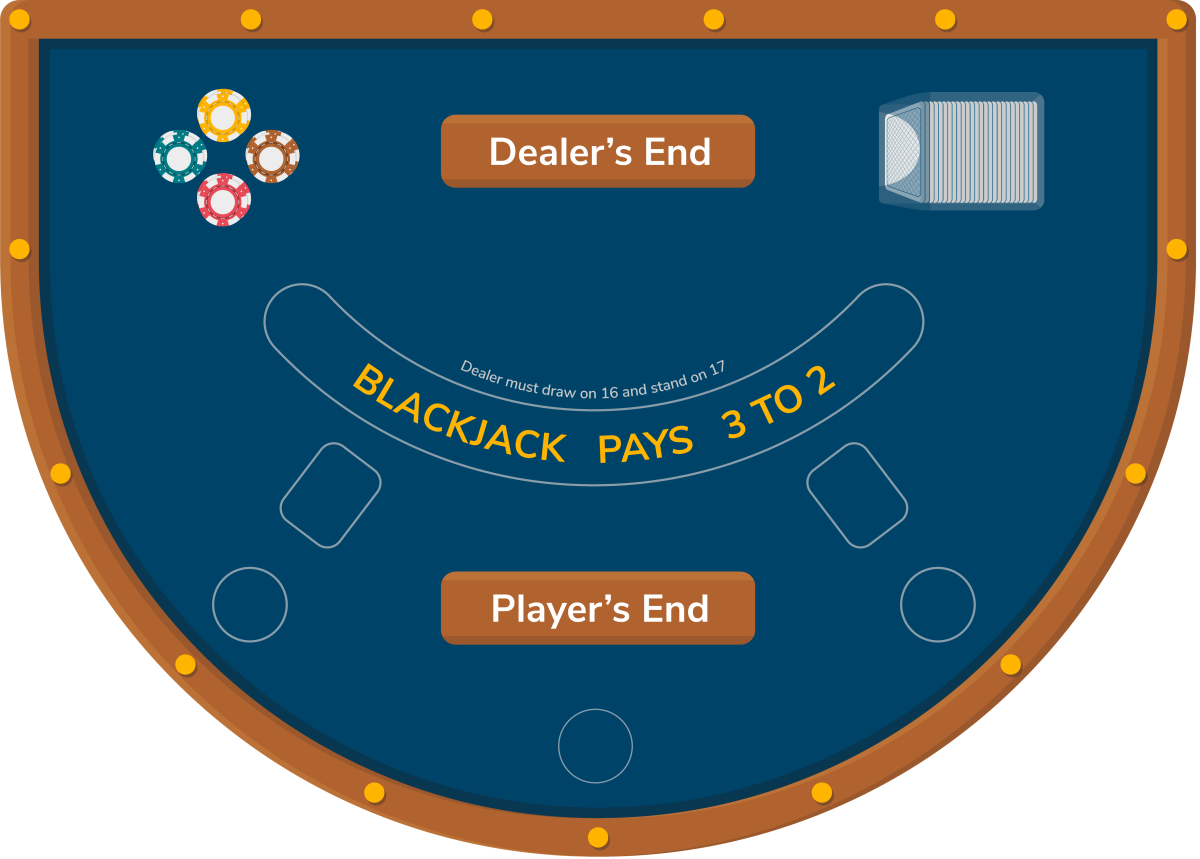
\includegraphics[width=\textwidth]{Images/chapter_12/section_5784621407272960/6297780793638912.png}
 \caption{The dealer’s end and player’s end}
 \end{subfigure}
\end{figure}

\begin{figure}[htbp]
 \centering
 \begin{subfigure}[b]{0.48\textwidth}
 \centering
 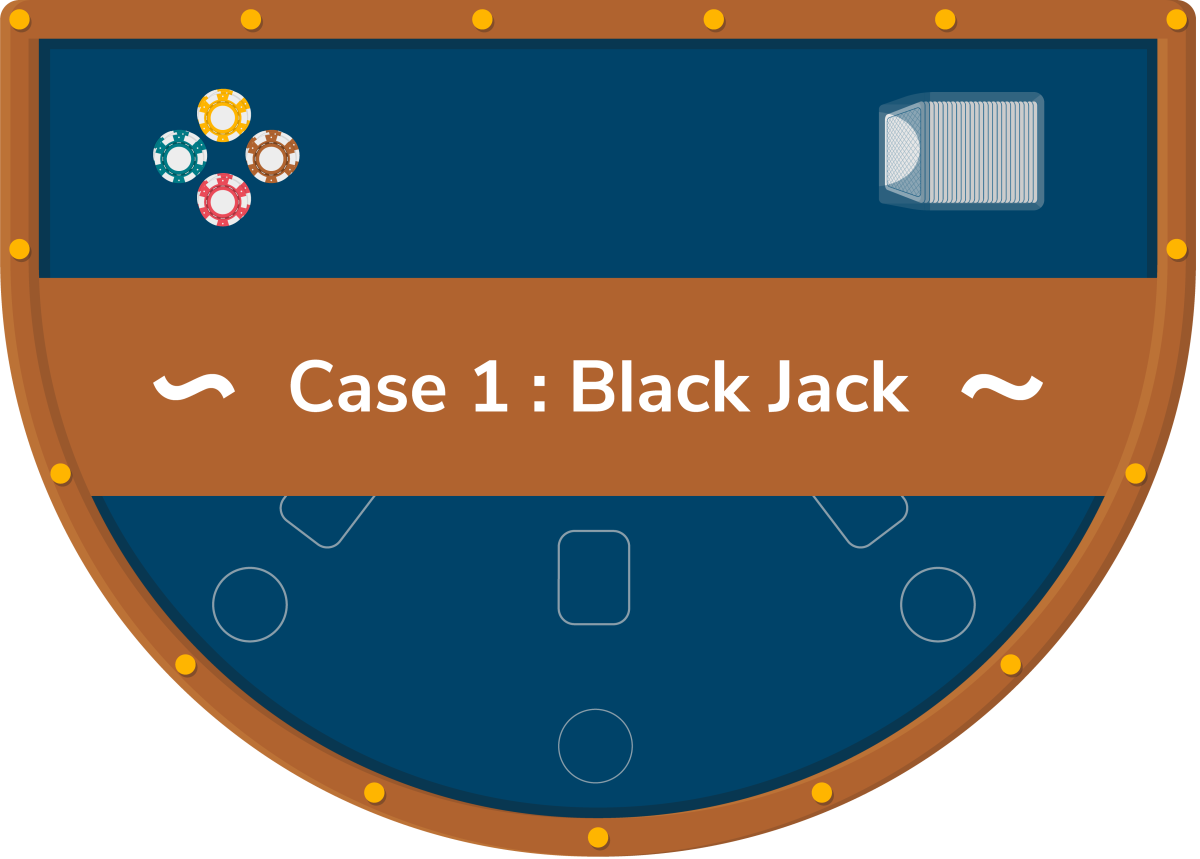
\includegraphics[width=\textwidth]{Images/chapter_12/section_5784621407272960/5498968567185408.png}
 \caption{Blackjack case represents if the player's first two cards’ sum is equal to 21 }
 \end{subfigure}
 \hfill
 \begin{subfigure}[b]{0.48\textwidth}
 \centering
 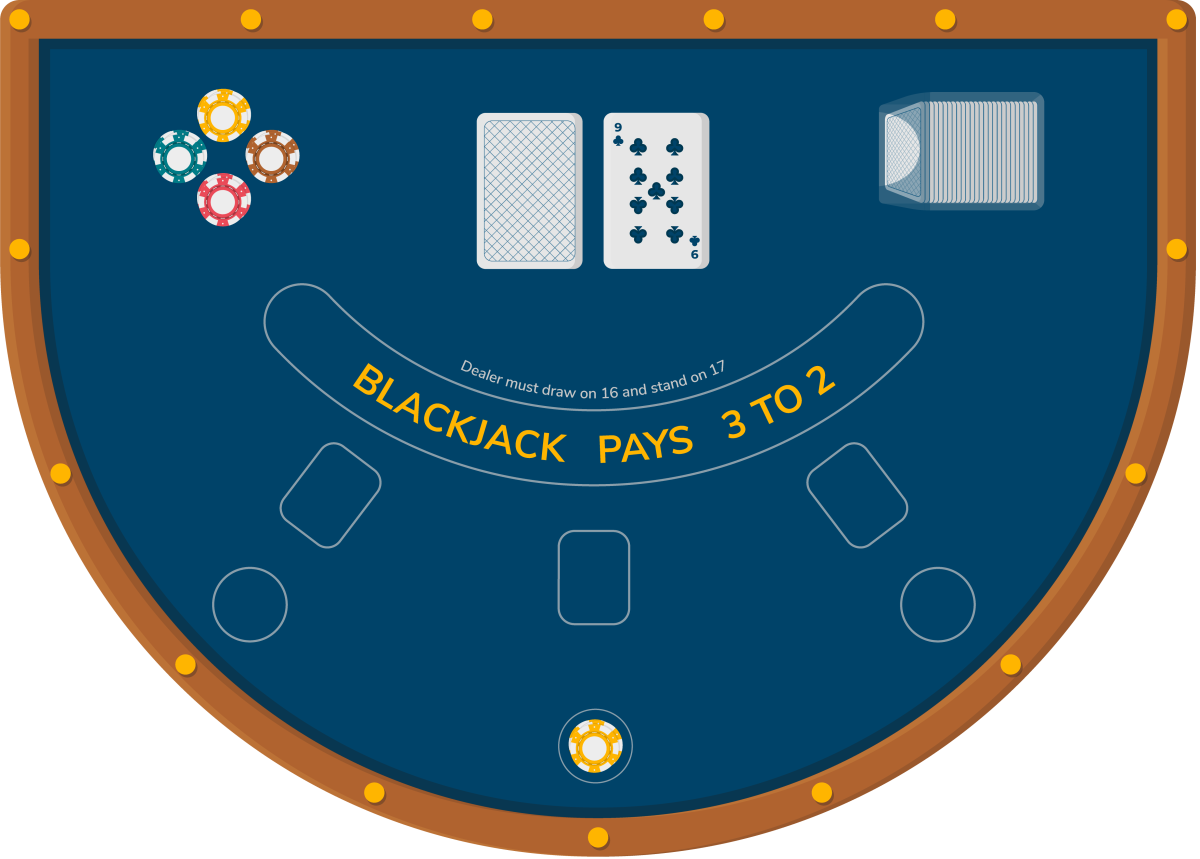
\includegraphics[width=\textwidth]{Images/chapter_12/section_5784621407272960/6145241151438848.png}
 \caption{The dealer deals two cards to themselves, one card facing up and the other card facing down}
 \end{subfigure}
\end{figure}

\begin{figure}[htbp]
 \centering
 \begin{subfigure}[b]{0.48\textwidth}
 \centering
 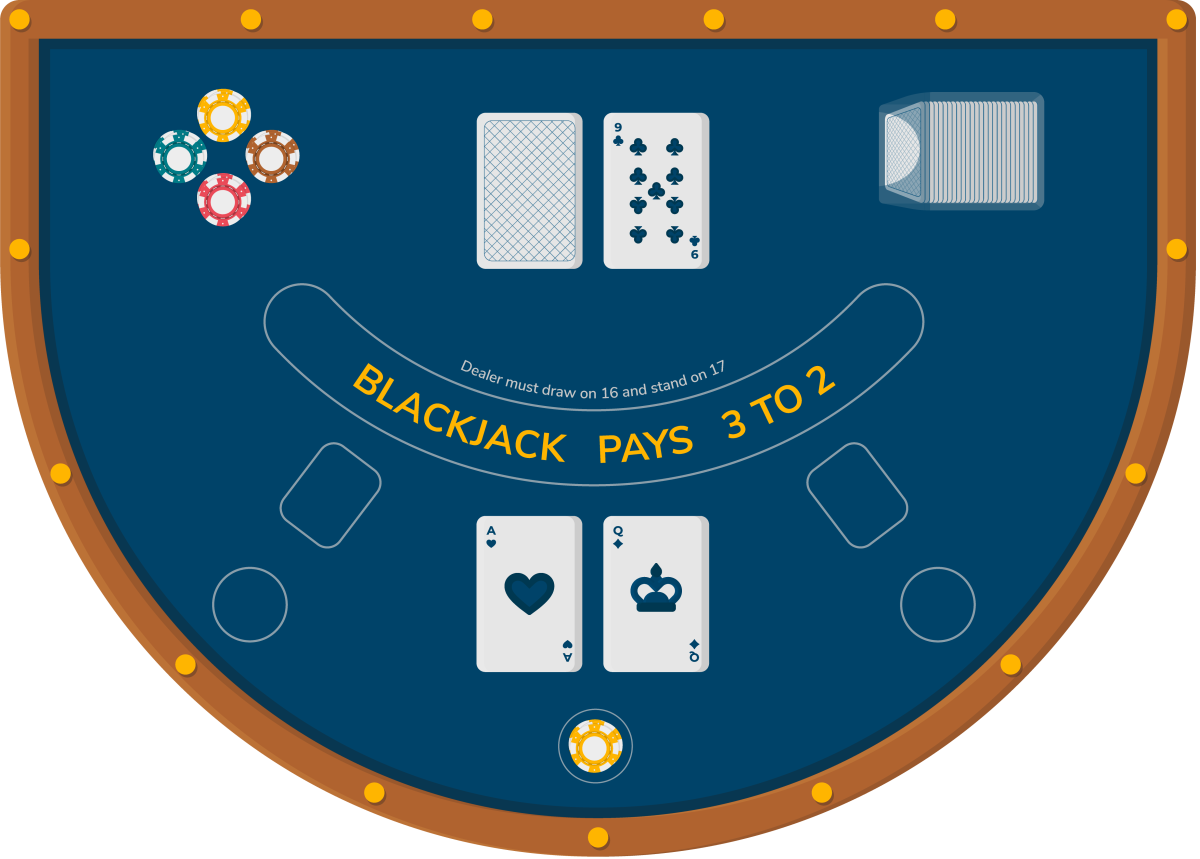
\includegraphics[width=\textwidth]{Images/chapter_12/section_5784621407272960/6358352767746048.png}
 \caption{The dealer will deal two cards to player (both cards facing up)}
 \end{subfigure}
 \hfill
 \begin{subfigure}[b]{0.48\textwidth}
 \centering
 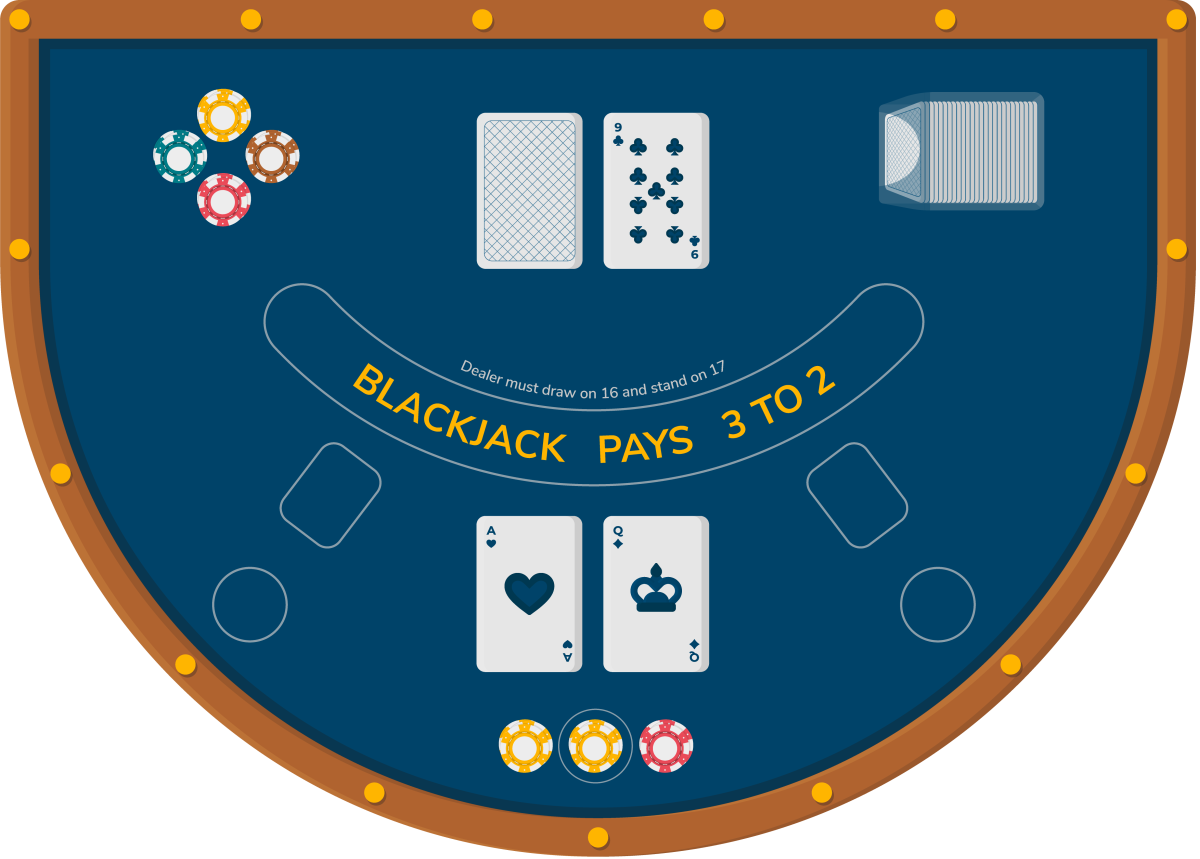
\includegraphics[width=\textwidth]{Images/chapter_12/section_5784621407272960/5681822434590720.png}
 \caption{Player wins the game because their first two cards' sum is equal to 21 and gets 150 percent profit}
 \end{subfigure}
\end{figure}

\begin{figure}[htbp]
 \centering
 \begin{subfigure}[b]{0.48\textwidth}
 \centering
 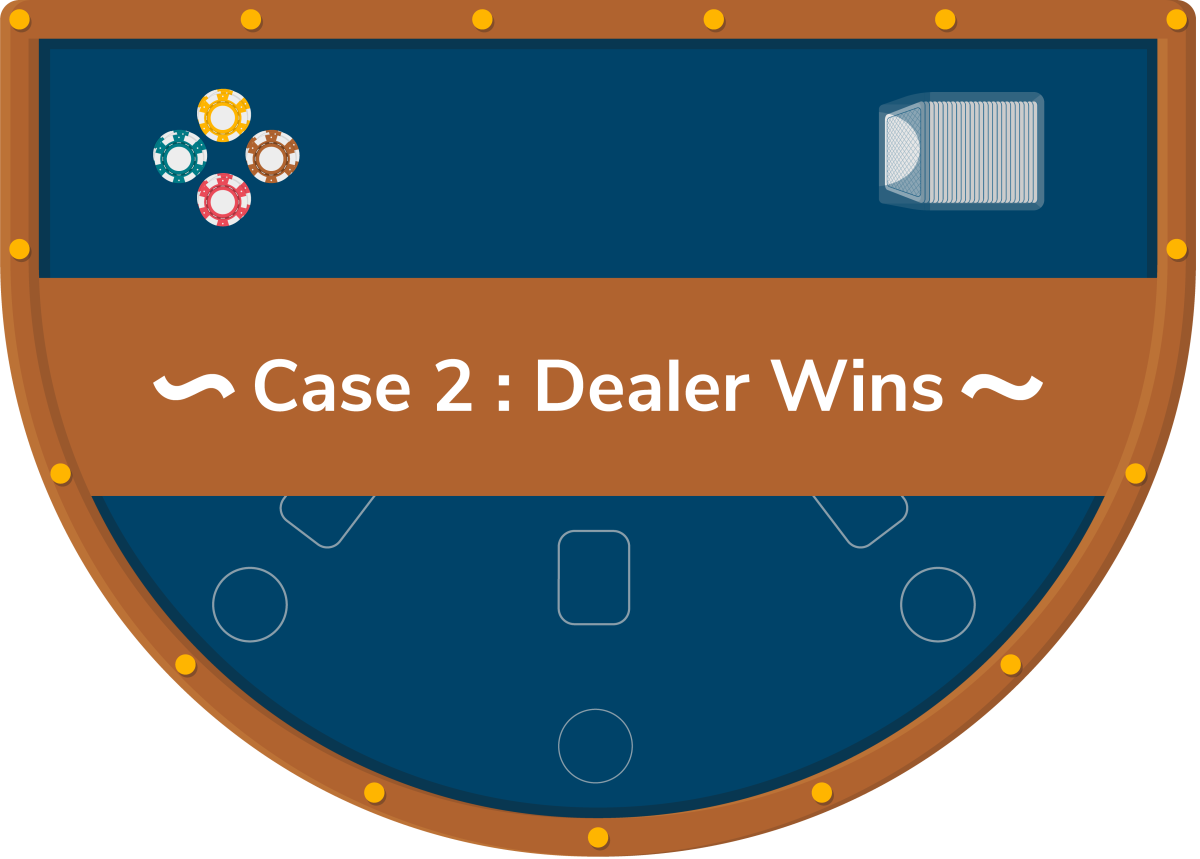
\includegraphics[width=\textwidth]{Images/chapter_12/section_5784621407272960/5494758221021184.png}
 \caption{Dealer wins if the dealer card sum is greater than player's card sum}
 \end{subfigure}
 \hfill
 \begin{subfigure}[b]{0.48\textwidth}
 \centering
 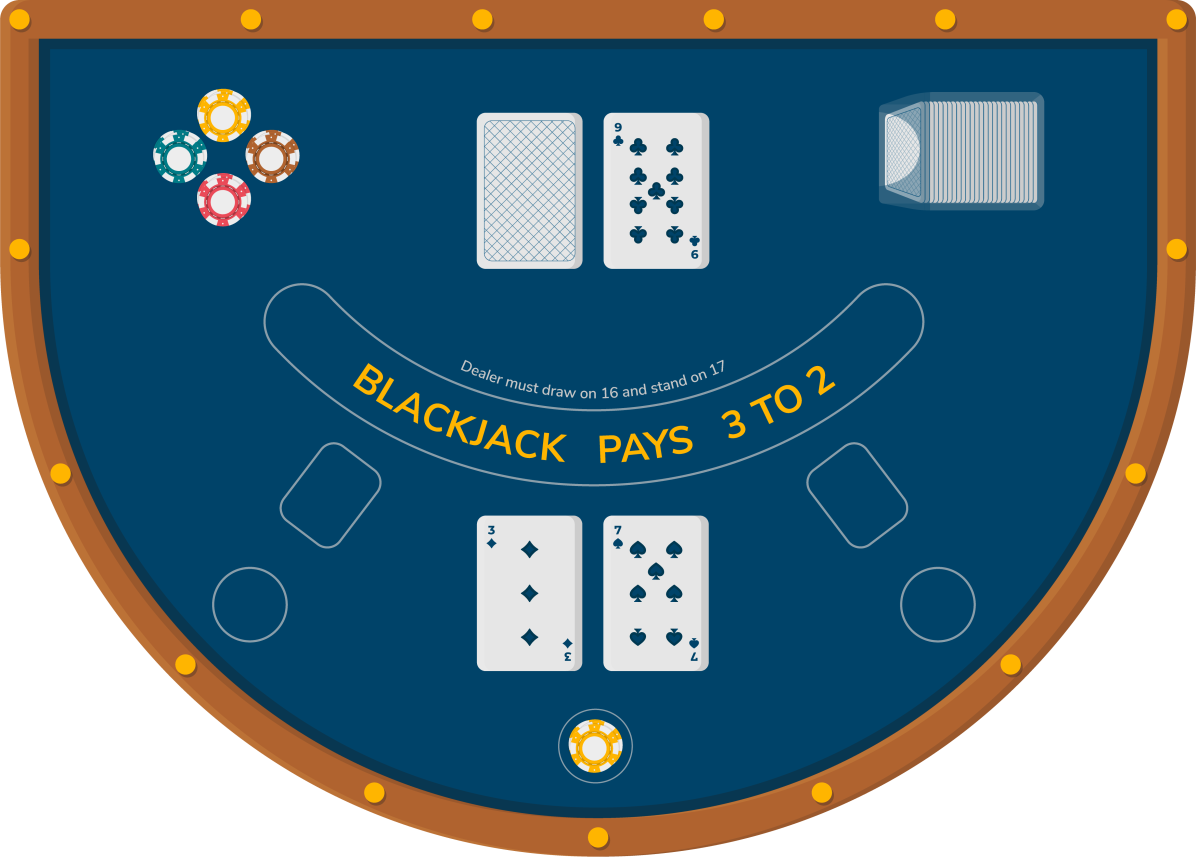
\includegraphics[width=\textwidth]{Images/chapter_12/section_5784621407272960/5028037144084480.png}
 \caption{The dealer deals two cards to themselves and two cards to the player}
 \end{subfigure}
\end{figure}

\begin{figure}[htbp]
 \centering
 \begin{subfigure}[b]{0.48\textwidth}
 \centering
 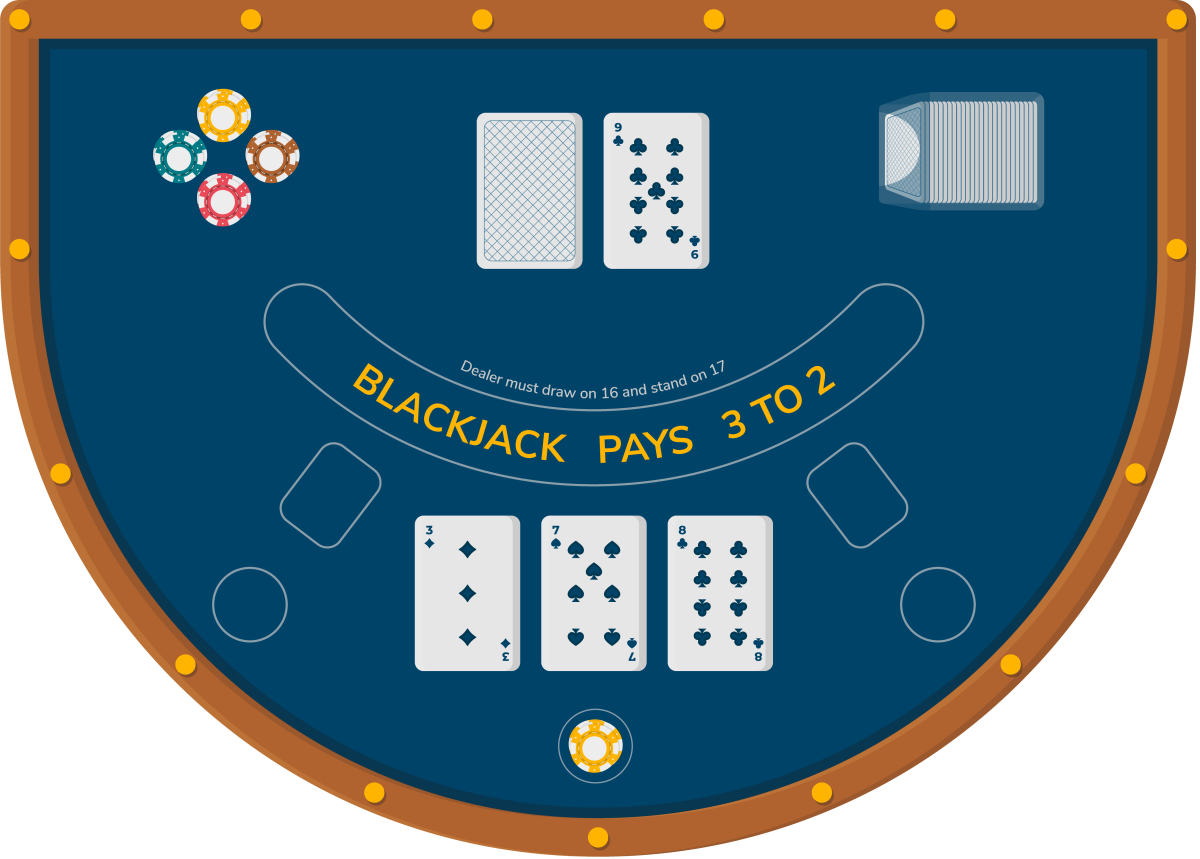
\includegraphics[width=\textwidth]{Images/chapter_12/section_5784621407272960/5032084533149696.png}
 \caption{The player hits and draws an additional card (8)}
 \end{subfigure}
 \hfill
 \begin{subfigure}[b]{0.48\textwidth}
 \centering
 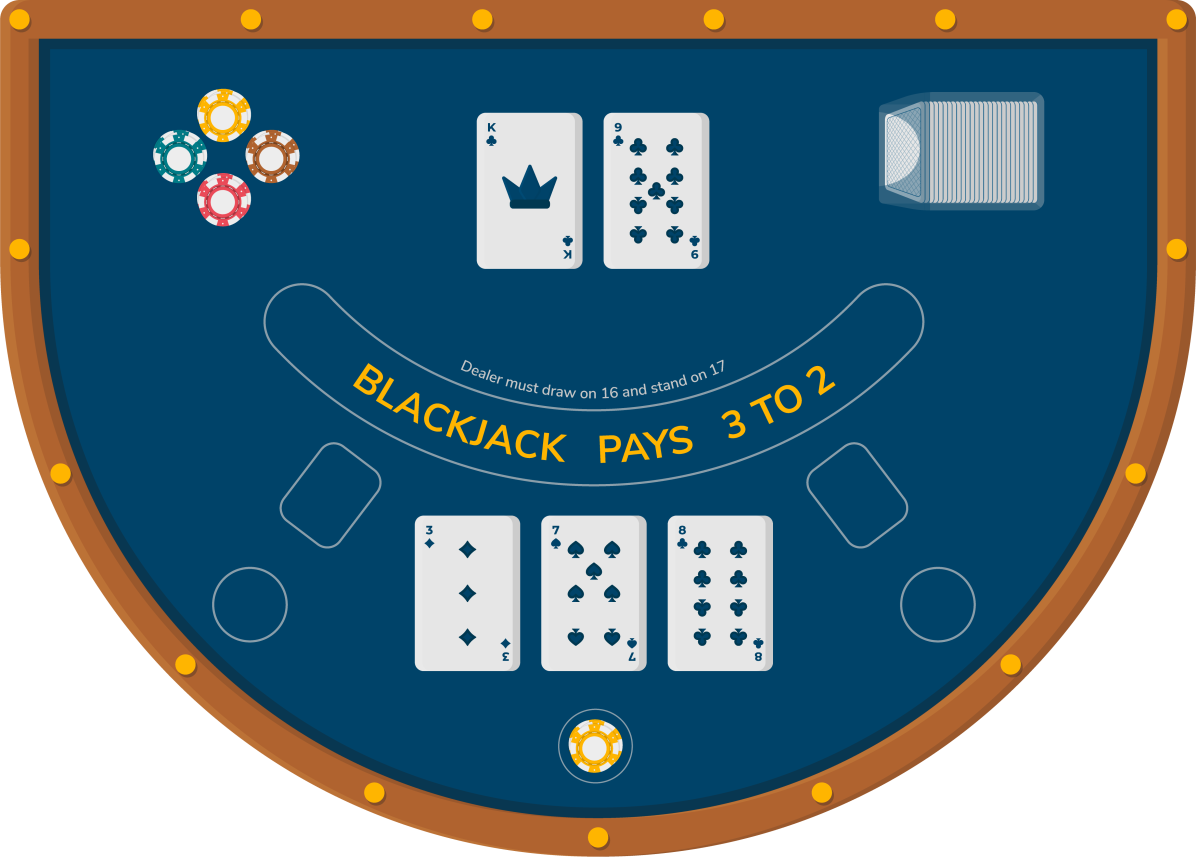
\includegraphics[width=\textwidth]{Images/chapter_12/section_5784621407272960/5001099783438336.png}
 \caption{After the player stands, the dealer exposes their second card }
 \end{subfigure}
\end{figure}

\begin{figure}[htbp]
 \centering
 \begin{subfigure}[b]{0.48\textwidth}
 \centering
 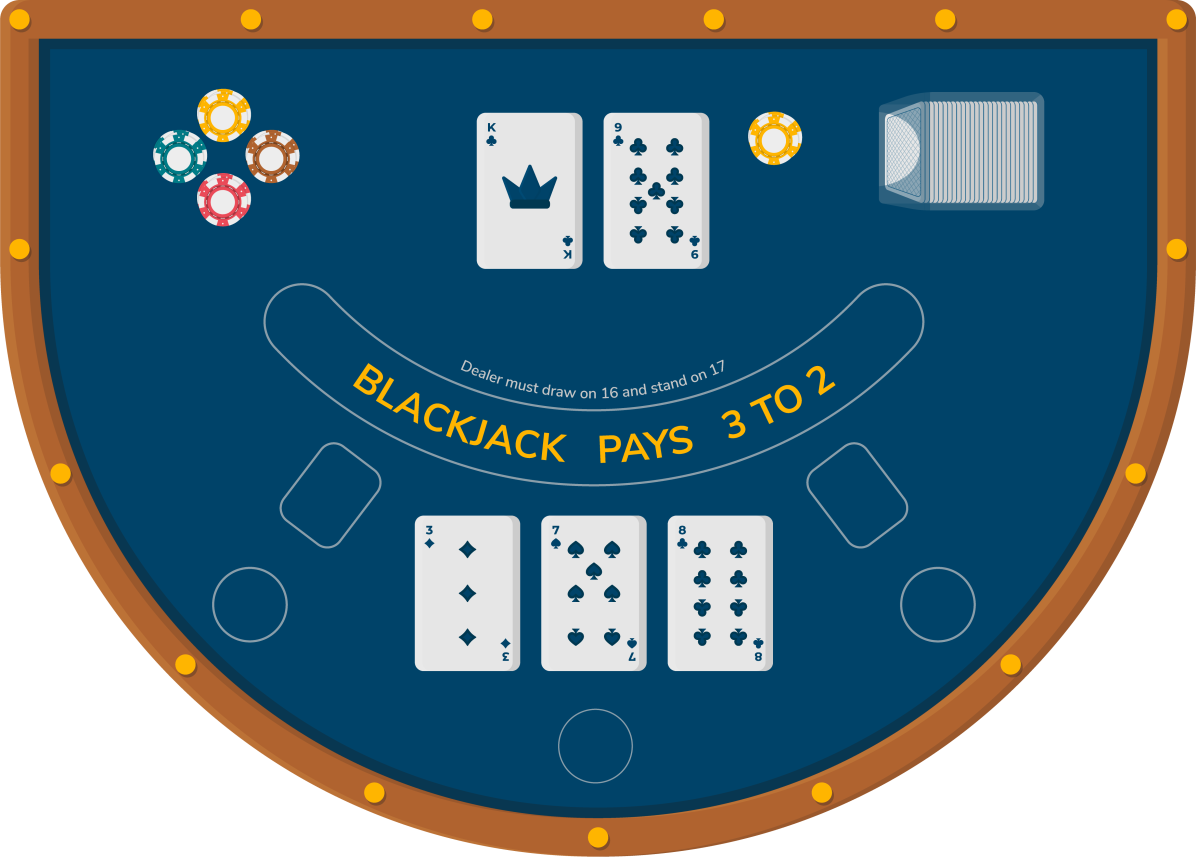
\includegraphics[width=\textwidth]{Images/chapter_12/section_5784621407272960/6422263052369920.png}
 \caption{Player loses the game and the bet because player cards’ sum (18) is less than dealer cards’ sum (19)}
 \end{subfigure}
 \hfill
 \begin{subfigure}[b]{0.48\textwidth}
 \centering
 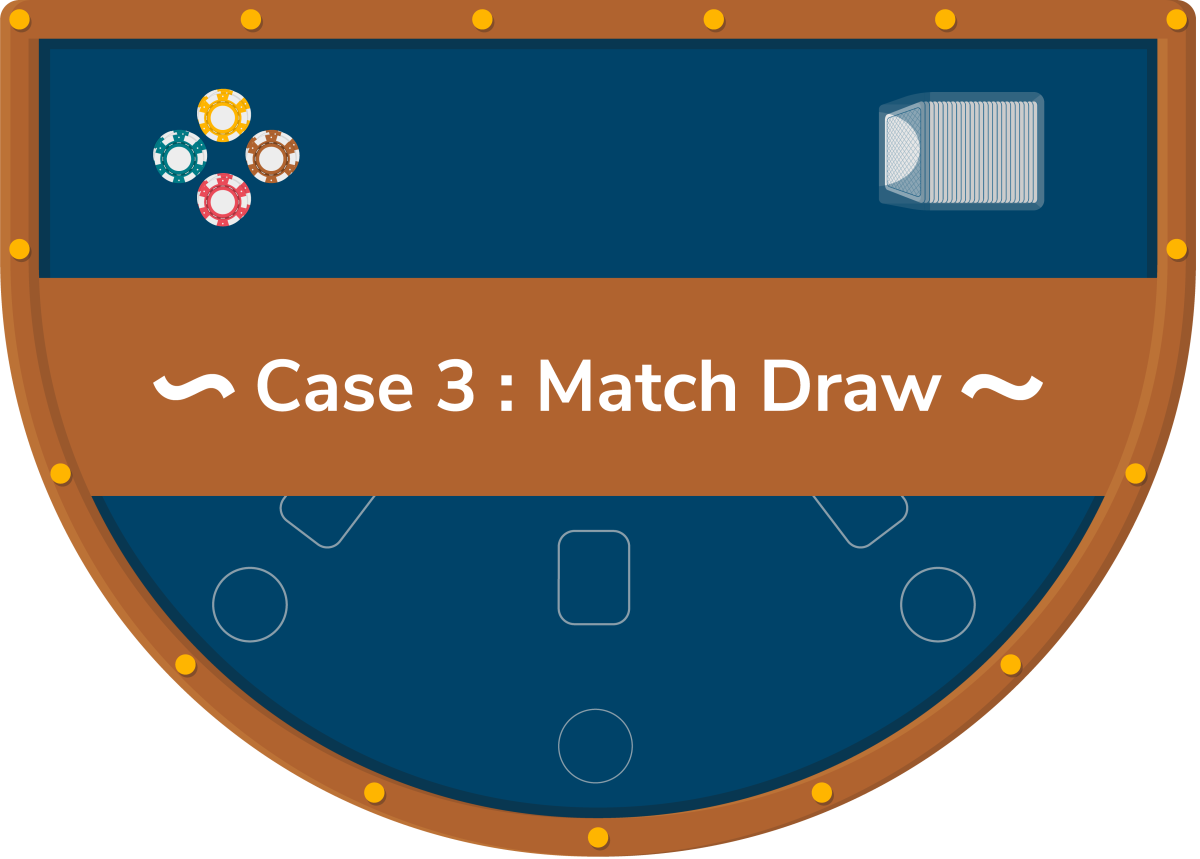
\includegraphics[width=\textwidth]{Images/chapter_12/section_5784621407272960/4539101996122112.png}
 \caption{The game results in a draw if the player card sum is equal to the dealer card sum}
 \end{subfigure}
\end{figure}

\begin{figure}[htbp]
 \centering
 \begin{subfigure}[b]{0.48\textwidth}
 \centering
 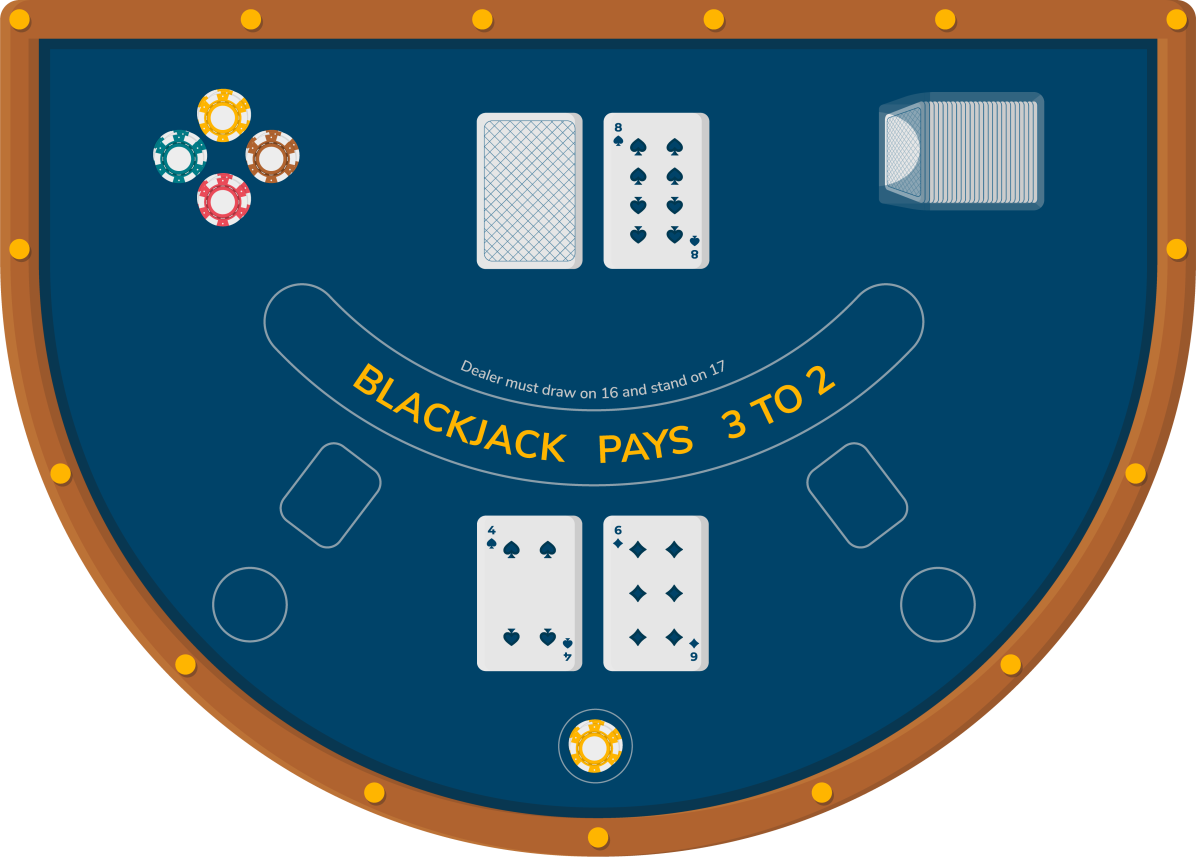
\includegraphics[width=\textwidth]{Images/chapter_12/section_5784621407272960/6105400769511424.png}
 \caption{The dealer deals two cards to themselves and two cards to the player}
 \end{subfigure}
 \hfill
 \begin{subfigure}[b]{0.48\textwidth}
 \centering
 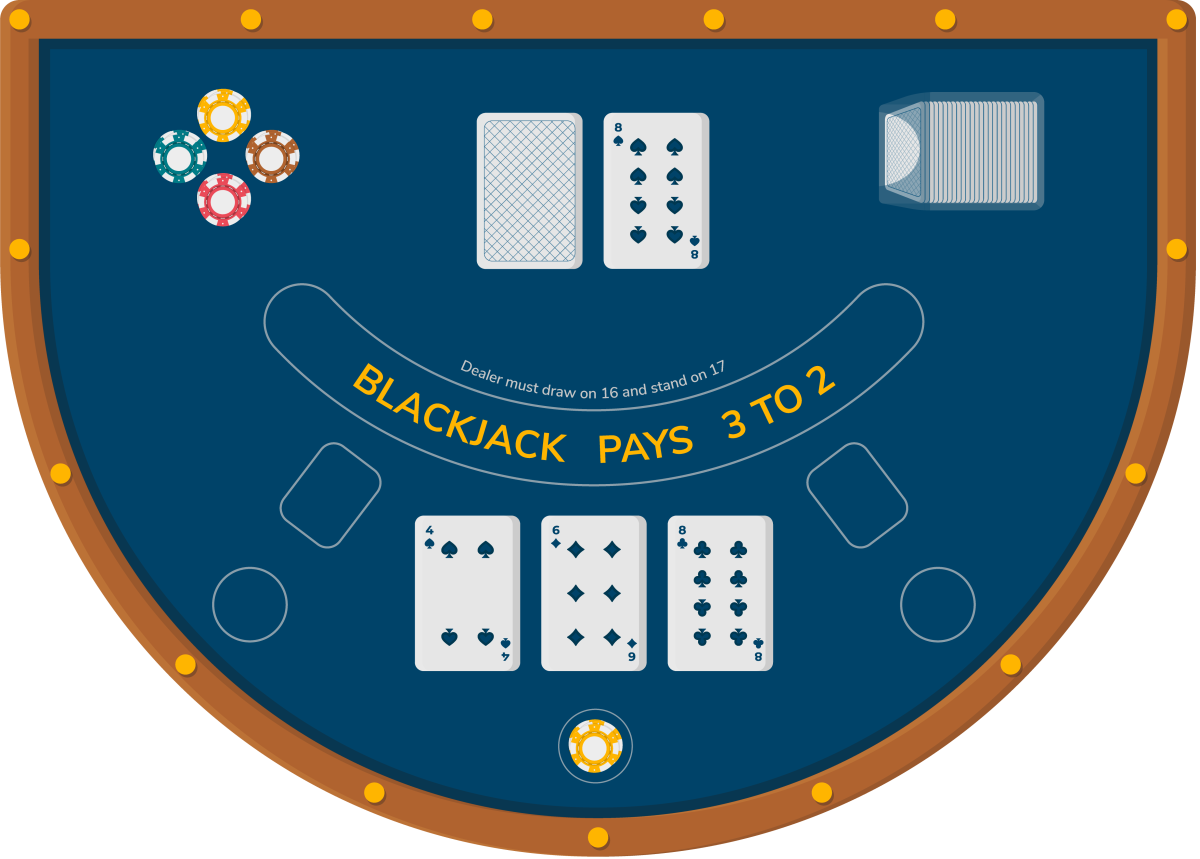
\includegraphics[width=\textwidth]{Images/chapter_12/section_5784621407272960/6539486520672256.png}
 \caption{The player hits and draws an additional card (8)}
 \end{subfigure}
\end{figure}

\begin{figure}[htbp]
 \centering
 \begin{subfigure}[b]{0.48\textwidth}
 \centering
 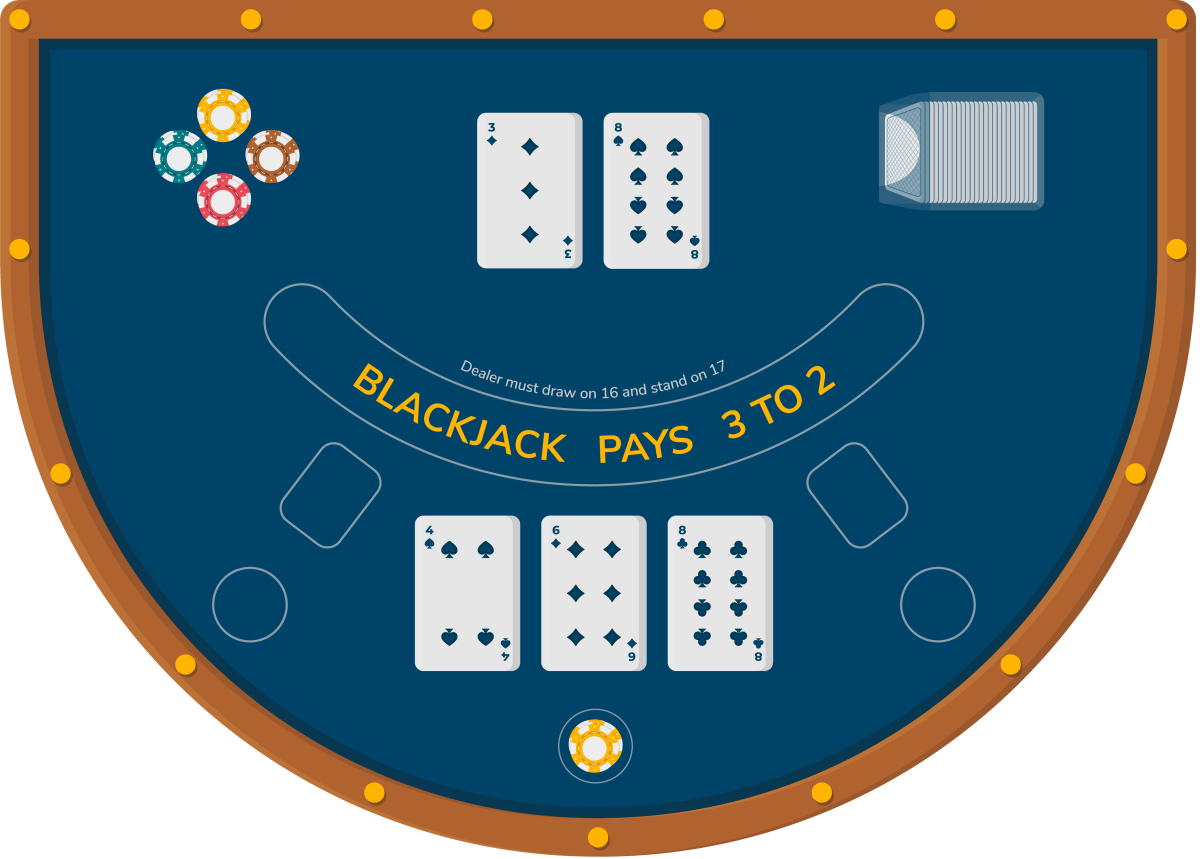
\includegraphics[width=\textwidth]{Images/chapter_12/section_5784621407272960/5936519434207232.png}
 \caption{After the player stands, the dealer exposes their second card }
 \end{subfigure}
 \hfill
 \begin{subfigure}[b]{0.48\textwidth}
 \centering
 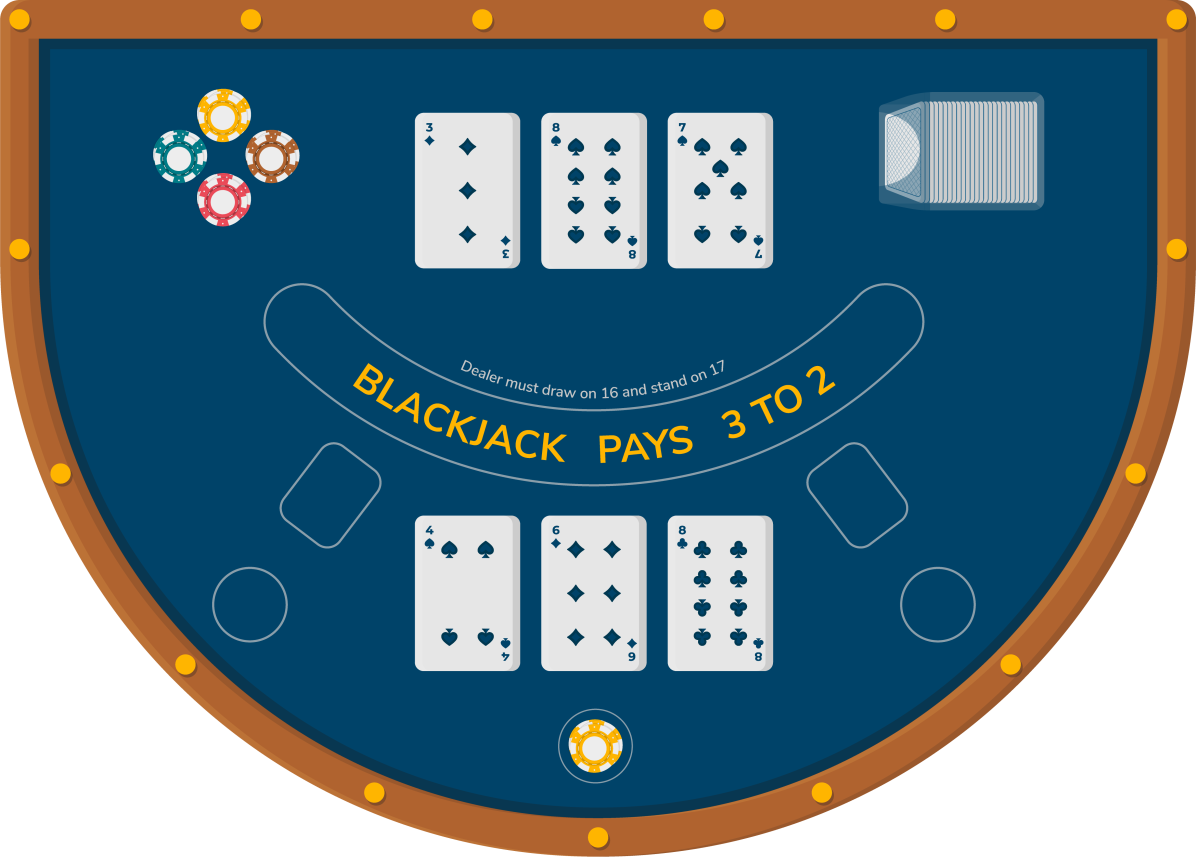
\includegraphics[width=\textwidth]{Images/chapter_12/section_5784621407272960/5314607498657792.png}
 \caption{The game results in a draw because player cards’ sum (18) is equal to the dealer cards’ sum (18)}
 \end{subfigure}
\end{figure}

\begin{figure}[htbp]
 \centering
 \begin{subfigure}[b]{0.48\textwidth}
 \centering
 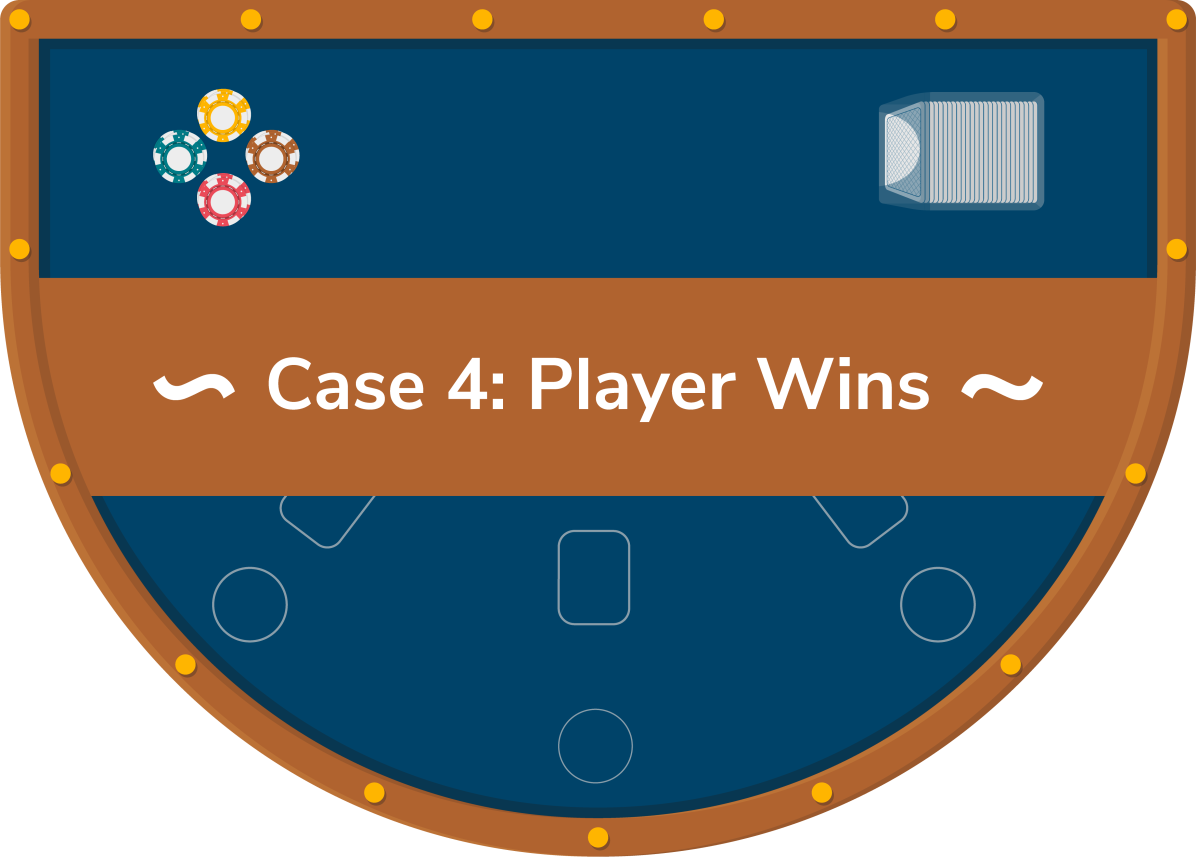
\includegraphics[width=\textwidth]{Images/chapter_12/section_5784621407272960/4762976324419584.png}
 \caption{The player wins if their card sum is greater than the dealer card sum}
 \end{subfigure}
 \hfill
 \begin{subfigure}[b]{0.48\textwidth}
 \centering
 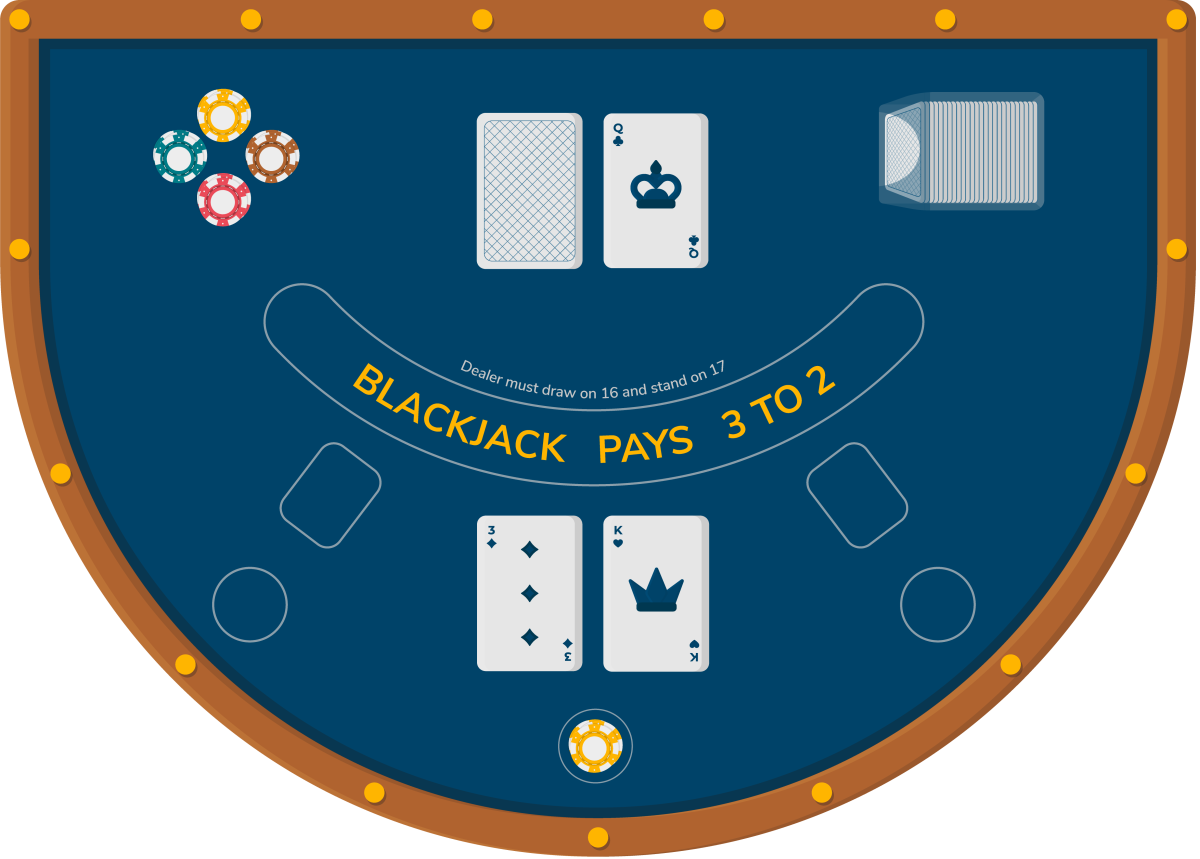
\includegraphics[width=\textwidth]{Images/chapter_12/section_5784621407272960/6656487134068736.png}
 \caption{The dealer deals two cards to themselves and two cards to the player}
 \end{subfigure}
\end{figure}

\begin{figure}[htbp]
 \centering
 \begin{subfigure}[b]{0.48\textwidth}
 \centering
 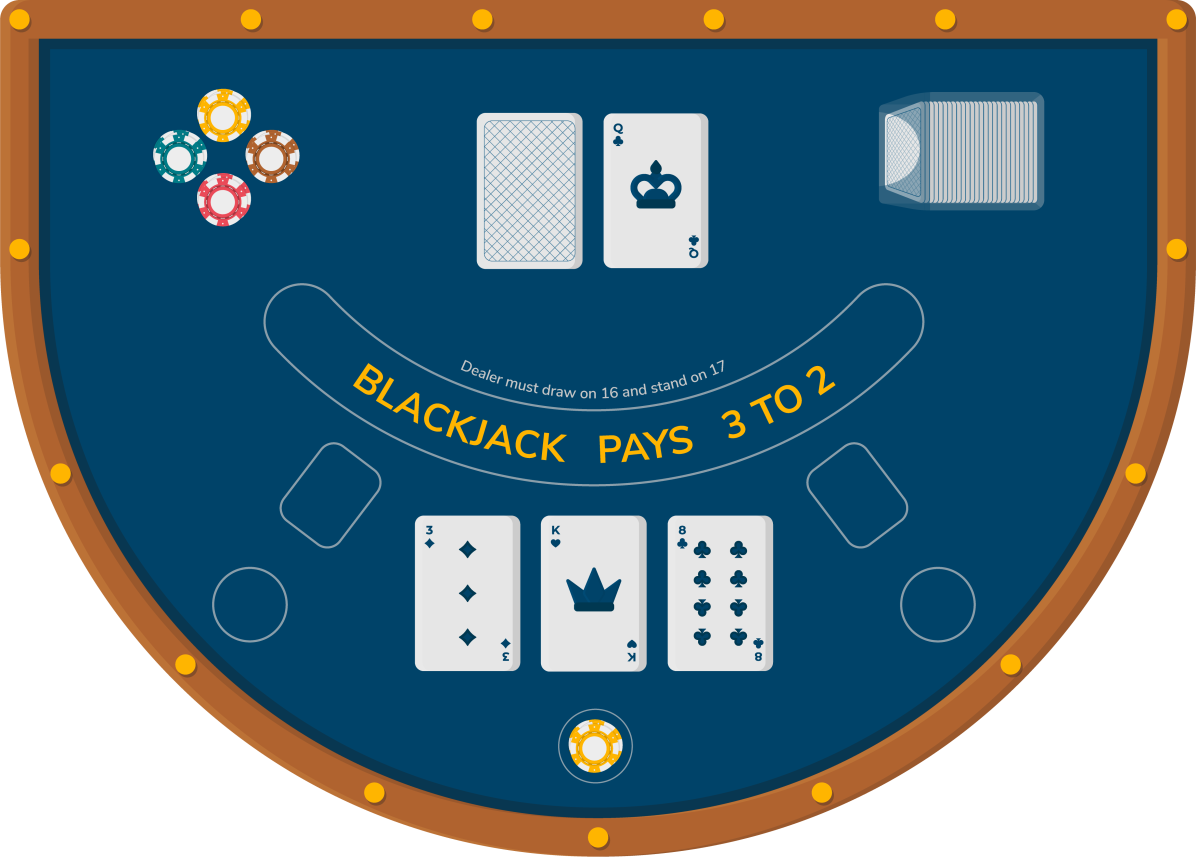
\includegraphics[width=\textwidth]{Images/chapter_12/section_5784621407272960/5815538107547648.png}
 \caption{The player hits and draws an additional card (8)}
 \end{subfigure}
 \hfill
 \begin{subfigure}[b]{0.48\textwidth}
 \centering
 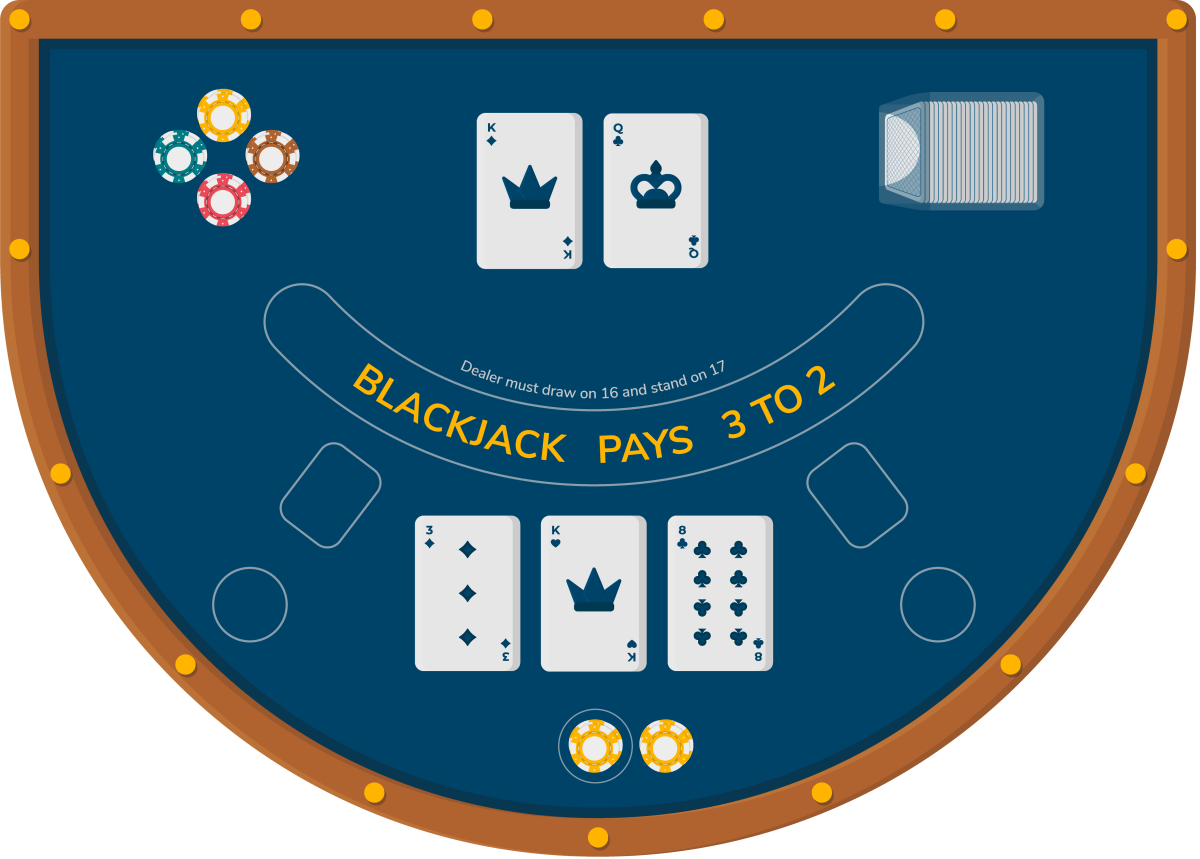
\includegraphics[width=\textwidth]{Images/chapter_12/section_5784621407272960/4743809750794240.png}
 \caption{The player wins the game and the bet( 100\%) because player cards sum is greater than the dealer cards sum}
 \end{subfigure}
\end{figure}

\subsection{Expectations from the interviewee}\label{KfyitG1dioESlbYIcgWus-2}
\\
There are several components in a Blackjack game, each with specific constraints and requirements. The following provides an overview of some of the main expectations that the interviewer will want to hear you discuss in more detail during the interview.

\subsubsection{Players in the game}\label{axGEKWE7_JQ1jSrAUevYe}
\\
To get a better understanding of the game and the players of the game, you may ask the interviewer the following set of questions:

\begin{enumerate}
\item
\protect\phantomsection\label{5AF1QHxagfvJeaiZSM4XE}
How many players can play Blackjack?
\item
\protect\phantomsection\label{HsuA53prXMJI9_nIG5P7S}
Can players play the game against each other?
\end{enumerate}

\subsubsection{Point dynamics}\label{XFsXY3tSOqI7cdXO8-q-G}
\\
The rules related to the number of points also need to be clarified by the interviewer; therefore, you may ask the questions listed below:

\begin{enumerate}
\item
How many points can the player or the dealer hit the card?
\item
What will happen if the dealer and the player get the same points?
\end{enumerate}

\subsubsection{Card limit}\label{fo2Lgz1_AiiYBhf1BfkEc}
\\
The interviewer would expect you to ask about the maximum number of cards the player can have. Therefore, you may ask a question listed below:

\begin{enumerate}
\item
Is there a limit on the number of cards the player takes?
\end{enumerate}

\subsection{Design approach}\label{nMxzgcL9_8ud3YtB3Weie}
\\
We will design this online Blackjack game using a bottom-up design approach. To achieve this, we will follow these steps:

\begin{itemize}
\item
First, we'll identify and design the smallest, core entities such as \texttt{Card}, \texttt{Hand}, and \texttt{Player} (including the dealer as a special player), clarifying their responsibilities and interactions.
\item
Next, we'll model the \texttt{Deck}, \texttt{GameTable}, and \texttt{GameController} to coordinate the game flow---dealing, betting, player actions, dealer logic, and determining results.
\item
We will incorporate game rules (card values, Blackjacks, busts, and win conditions) into these entities' behaviors, ensuring correctness and clarity.
\item
We'll ensure that the design allows for scalability, supporting multiple tables and concurrent games, and enforcing a clear separation of concerns for easy maintenance and extension.
\item
We'll highlight how SOLID principles and relevant design patterns can help us achieve a clean, maintainable system.
\end{itemize}

\subsection{Design pattern~}\label{ZrZ5MDGLUDSdWp0KcJgGF}
\\
During an interview, discussing the design patterns that an online Blackjack game falls under is always a good practice. Stating the design patterns gives the interviewer a positive impression and shows that the interviewee is well-versed in the advanced concepts of object-oriented design.
\\
Try to answer the following question. If you are not familiar with design patterns, don't worry! You can learn about them by asking, ``Define design patterns.''

\textbf{Question:}

Which design pattern(s) should be used to design an online Blackjack game? Please elaborate on your choice(s).

Let's explore the requirements of the online Blackjack game in the next lesson.

\subsection{}\label{d3Pm1FQEShUrw4RLRwW-a}

% End of section content